\documentclass[11pt,border=5pt]{standalone}
\usepackage{amsmath,amssymb,graphicx,enumitem}
\setlength{\parindent}{0pt}
\setlength{\parskip}{4pt}
\setlength{\abovedisplayskip}{5pt}
\setlength{\belowdisplayskip}{5pt}
\setlength{\abovedisplayshortskip}{3pt}
\setlength{\belowdisplayshortskip}{3pt}
\setlist[itemize]{leftmargin=13pt,labelsep=4pt,itemsep=2pt,topsep=3pt,parsep=0pt}
\newcommand{\stepheading}[1]{\par\vspace{5pt}\textbf{#1}\par}
\newcommand{\magnitudeformula}{%
  \begin{gathered}
  |H(e^{j\Omega})|={}\\[2pt]
  \dfrac{1}{\sqrt{1.89-0.2\cos\Omega-1.6\cos(2\Omega)}}
  \end{gathered}}
\begin{document}
\begin{minipage}{260pt}
\begin{center}
{\large\bfseries Question 3(c) --\\[2pt]
Amplitude magnification}
\end{center}
\vspace{-3pt}

(c) Amplitude magnification \( |H(e^{j\Omega})| \)

We are given
\[
\begin{aligned}
H(e^{j\Omega})
&=\frac{1}{1-0.5e^{-j\Omega}-0.8e^{-j2\Omega}}\\[5pt]
&=\frac{e^{j2\Omega}}{e^{j2\Omega}-0.5e^{j\Omega}-0.8}.
\end{aligned}
\]

\stepheading{Step 1: Take the magnitude}
Since
\[
|e^{j2\Omega}|=1,
\]
the numerator does not affect the magnitude, so
\[
\begin{gathered}
|H(e^{j\Omega})|={}\\[2pt]
\frac{1}{\left|1-0.5e^{-j\Omega}-0.8e^{-j2\Omega}\right|}.
\end{gathered}
\]

\stepheading{Step 2: Simplify the denominator magnitude}
Let
\[
D(\Omega)=1-0.5e^{-j\Omega}-0.8e^{-j2\Omega}.
\]
Then
\[
|H(e^{j\Omega})|
=\frac{1}{\sqrt{D(\Omega)D^*(\Omega)}}.
\]
This simplifies to
\[
\magnitudeformula.
\]
So the amplitude magnification is
\[
\boxed{\magnitudeformula}
\]

\stepheading{Step 3: Compute a few key points for the sketch}
At \(\Omega=0\)
\[
\begin{aligned}
|H(e^{j0})|
&=\frac{1}{|1-0.5-0.8|}\\[4pt]
&=\frac{1}{0.3}\approx 3.33
\end{aligned}
\]

At \(\Omega=\frac{\pi}{2}\)
\[
\cos\left(\frac{\pi}{2}\right)=0,
\qquad\cos(\pi)=-1
\]
\[
\begin{aligned}
|H(e^{j\pi/2})|
&=\frac{1}{\sqrt{1.89-0-1.6(-1)}}\\[4pt]
&=\frac{1}{\sqrt{3.49}}\approx 0.54
\end{aligned}
\]

At \(\Omega=\pi\)
\[
\cos(\pi)=-1,\qquad\cos(2\pi)=1
\]
\[
\begin{gathered}
|H(e^{j\pi})|={}\\[2pt]
\begin{aligned}
&\frac{1}{\sqrt{1.89-0.2(-1)-1.6(1)}}\\[4pt]
&\quad=\frac{1}{\sqrt{0.49}}
=\frac{1}{0.7}\approx 1.43
\end{aligned}
\end{gathered}
\]

At \(\Omega=\frac{3\pi}{2}\)
\[
|H(e^{j3\pi/2})|\approx 0.54
\]

At \(\Omega=2\pi\)
\[
|H(e^{j2\pi})|\approx 3.33
\]

\stepheading{Step 4: Important shape information}
So the curve:
\begin{itemize}
\item starts high at \(\Omega=0\)
\item drops to a minimum near \(\Omega=\pi/2\)
\item rises again to a smaller peak at \(\Omega=\pi\)
\item drops again near \(\Omega=3\pi/2\)
\item rises back to a high value at \(\Omega=2\pi\)
\end{itemize}

Key values:
\[
\boxed{\begin{aligned}
|H(e^{j0})|&\approx 3.33\\[2pt]
|H(e^{j\pi/2})|&\approx 0.54\\[2pt]
|H(e^{j\pi})|&\approx 1.43\\[2pt]
|H(e^{j3\pi/2})|&\approx 0.54\\[2pt]
|H(e^{j2\pi})|&\approx 3.33
\end{aligned}}
\]

\stepheading{Sketch}
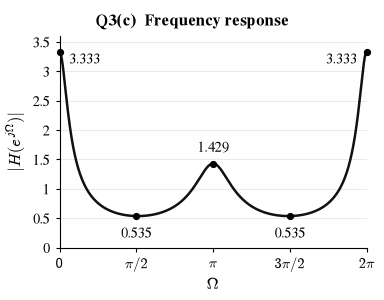
\includegraphics[width=\linewidth]{../../Q03c_frequency_response_384.png}

\stepheading{Final answer:}
\[
\boxed{\magnitudeformula}
\]
and the sketch has:
\begin{itemize}
\item a large peak at \(0\) and \(2\pi\) (\(\approx3.33\))
\item minima near \(\pi/2\) and \(3\pi/2\) (\(\approx0.54\))
\item a smaller peak at \(\pi\) (\(\approx1.43\))
\end{itemize}
\end{minipage}
\end{document}
